%%%%%%%%%%%%%%%%%%%%%%%%%%%%%%%%%%%%%%%%
\chapter{Resultados y discusión}
%%%%%%%%%%%%%%%%%%%%%%%%%%%%%%%%%%%%%%%%

%%%%%%%%%%%%%%%%%%%%%%%%%%%%%%%%%%%%%%%%
\section{Caracterización del corpus}

El proceso de selección PRISMA resultó en la inclusión de 84 estudios a partir de 140 registros identificados en Scopus. Las exclusiones en la Fase 2 correspondieron principalmente a artículos que no especificaban la tarea NLP ni el modelo base (Q4, n~=~16), con casos como predicción de trayectorias, clasificación de señales de sensores y regresión numérica sobre datos tabulares, seguido de técnicas fuera del alcance del estudio (Q2, n~=~7) y ausencia de resultados experimentales propios (Q5, n~=~1).

La clasificación de los 84 estudios en cuatro dominios de aplicación se realizó de forma automatizada durante la Fase 3, aplicando los criterios definidos en la sección de Metodología. La distribución resultante evidencia un marcado predominio del área de Salud y Biomedicina, con 30 estudios (35,7\%), seguido de Lenguaje y Humanidades con 21 (25,0\%), Ciencias Exactas y Computación con 20 (23,8\%) e Industria y Negocios con 13 (15,5\%). Esta distribución refleja la intensa actividad investigativa que el \textit{fine-tuning} de \textit{Large Language Models} ha tenido en aplicaciones clínicas y biomédicas durante el período 2020--2025, fenómeno concordante con la disponibilidad de corpus especializados como PubMed y MIMIC y con la demanda de modelos adaptados para tareas de extracción de información médica. La Figura~\ref{fig:dominios} presenta esta distribución de forma visual.

\begin{figure}[H]
    \centering
    \caption{Distribución del corpus por dominio de aplicación (n = 84)}
    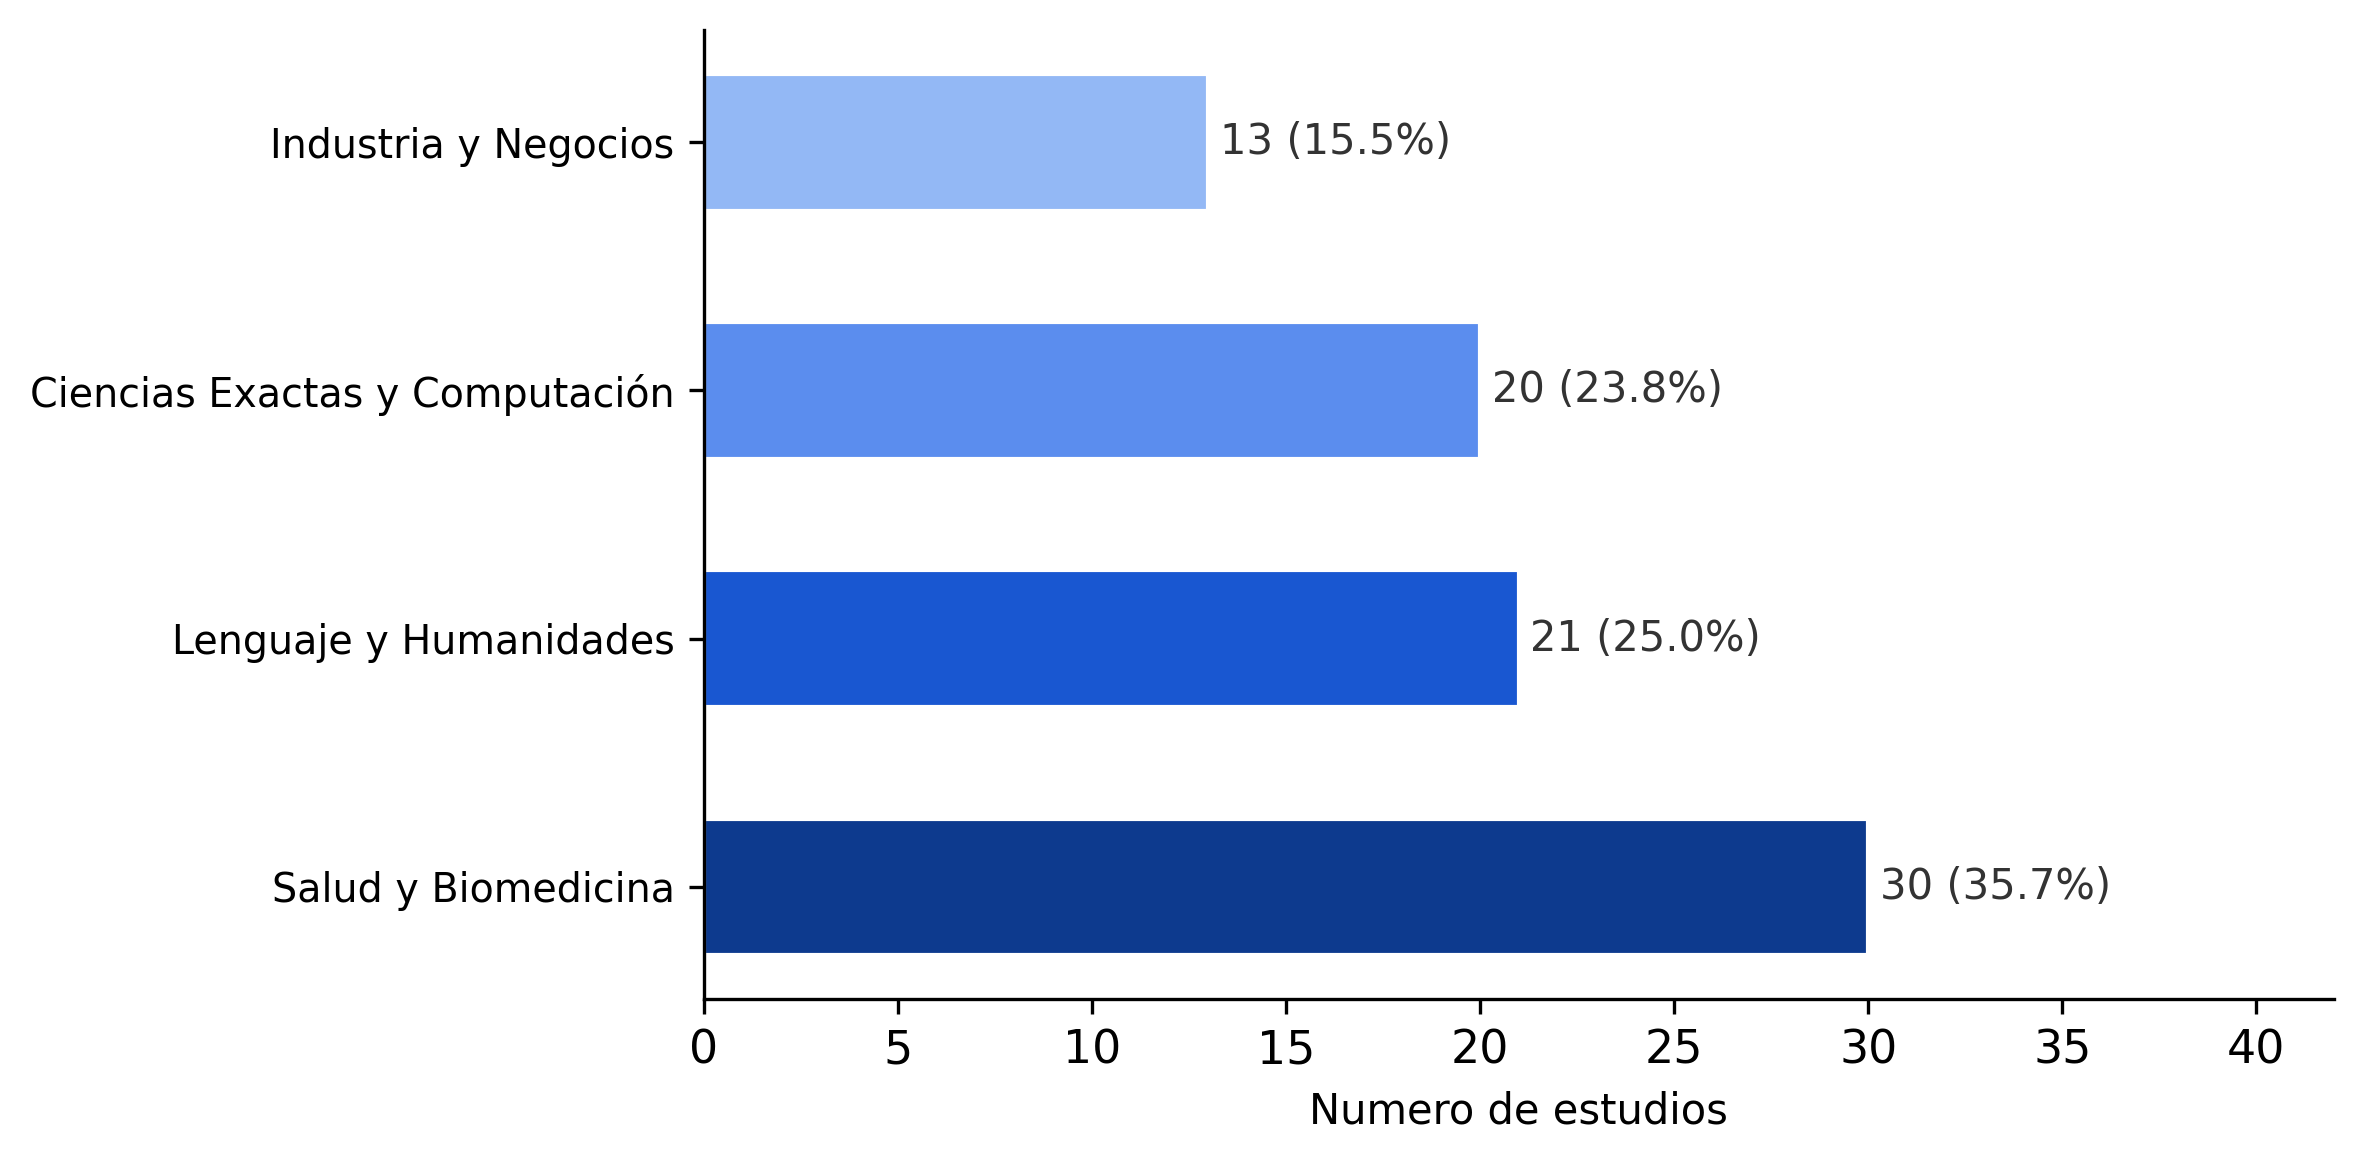
\includegraphics[width=0.85\linewidth]{Imagenes/fig2_distribucion_dominios.png}
    \label{fig:dominios}
\end{figure}

La calidad metodológica del corpus fue aceptable en conjunto: el \textit{score} promedio fue de 2,61 sobre 3,0, con la mayoría de estudios por encima del umbral de priorización de 2,5 establecido en la Metodología. A nivel de criterios individuales, QA4 obtuvo la puntuación media más alta, reflejando que prácticamente la totalidad de los estudios caracteriza con precisión sus \textit{datasets}. QA1 y QA3 presentaron medias más bajas, con una proporción menor de estudios que reportan \textit{splits} explícitos o que detallan de forma completa los hiperparámetros de entrenamiento. Por dominio, Lenguaje y Humanidades concentra la mayor calidad metodológica promedio, mientras que Industria y Negocios presenta la media más baja con la mayor variabilidad, lo que refleja heterogeneidad en las prácticas de reporte dentro de ese dominio.

%%%%%%%%%%%%%%%%%%%%%%%%%%%%%%%%%%%%%%%%
\section{Resultados por dominio}

%%%%%%%%%%%%%%%%%%%%%%%%%%%%%%%%%%%%%%%%
\subsection{Salud y Biomedicina}

El dominio de Salud y Biomedicina concentra 30 estudios, constituyendo el grupo más numeroso del corpus (35,7\%).

\subsubsection{Técnicas y modelos predominantes}

En este dominio, LoRA y QLoRA constituyen la categoría dominante con 21 de los 30 estudios (70,0\%), seguidas de técnicas alternativas como Adapters, Prefix Tuning y variantes con 5 estudios (16,7\%), \textit{Full Fine-Tuning} con 3 (10,0\%) y métodos de alineación con 1 (3,3\%). Dentro de la familia LoRA, dos estudios incorporan GRPO como mecanismo de alineación: educación cardiovascular \parencite{rullo2025cardio} y generación de reportes clínicos \parencite{kuo2025medical}. El único método de alineación es SFT+DPO para razonamiento clínico \parencite{savage2025dpo}. Técnicas alternativas como P-Tuning v2 \parencite{liu2024cpmi} y \textit{Prompt Tuning} \parencite{yang2025ceprompt} aparecen de forma puntual, reflejando que el dominio biomédico experimenta con distintos enfoques de adaptación paramétrica aunque LoRA concentra la mayoría de las aplicaciones.

\subsubsection{Tareas y métricas}

Las tareas identificadas en el dominio se agrupan en cuatro categorías principales. La extracción de información clínica (reconocimiento de entidades nombradas, extracción de medicamentos y relaciones) es la más frecuente, con estudios en NER médico en chino \parencite{zhou2024adapter} y extracción de medicamentos \parencite{richterpechanski2025medication}. Le siguen la respuesta a preguntas médicas y los sistemas de diálogo especializado \parencite{adhikary2025medical, bayram2025medical, tong2025xuanhugpt}, la generación y resumen de texto clínico \parencite{chao2025evaluating, hou2024ft} y la clasificación en salud pública, que abarca análisis de sentimiento \parencite{elmitwalli2024ft} y detección de desinformación \parencite{zhao2025daft}.

La heterogeneidad de métricas reportadas refleja directamente la diversidad de subtareas. En tareas de extracción y clasificación predominan F1 y sus variantes; en NER médico, por ejemplo, se reporta una mejora de F1 de 62,40\% a 65,90\% \parencite{zhou2024adapter}. En tareas de generación y resumen predominan ROUGE y BLEU, con ejemplos como la generación de cartas médicas \parencite{hou2024ft}. Una limitación recurrente en el corpus es la ausencia de un \textit{baseline} declarado explícitamente: varios estudios evalúan múltiples modelos o configuraciones y reportan el mejor resultado sin establecer una referencia de comparación fija, lo que impide atribuir la mejora a la técnica de \textit{fine-tuning} de forma aislada. De los 30 estudios, 9 reportan métricas cuantitativas comparables; los resultados detallados por estudio se presentan en la Tabla~\ref{tab:apx_salud} del Apéndice~A.

\subsubsection{Patrones de aplicabilidad}

Del análisis de los 30 estudios emergen tres patrones de aplicabilidad consistentes en el dominio.

El primero es la ventaja del \textit{fine-tuning} específico sobre el modelo base sin adaptar. Los estudios con resultados numéricos explícitos muestran que LoRA y QLoRA producen mejoras sustanciales sobre los \textit{baselines} de referencia en las subtareas evaluadas. Este patrón se observa en el dominio geriátrico, donde LLaMA3.1-8B ajustado sobre datos de cuidado especializado mejora de ROUGE 8,60\% a 34,96\% (+306,5\%) respecto al mismo modelo sin adaptar \parencite{xu2025cpel}, y en generación de cartas médicas, donde QLoRA mejora ROUGE-1 de 0,161 a 0,352 (+118,6\%) \parencite{hou2024ft}.

El segundo es la preferencia por modelos abiertos en entornos regulados. La imposibilidad de enviar datos clínicos sensibles a APIs externas condiciona directamente la elección de técnica y arquitectura. Al menos un estudio señala explícitamente que los modelos propietarios no pudieron ser evaluados porque las versiones seguras para datos clínicos protegidos no estaban disponibles al momento del estudio \parencite{chao2025evaluating}. Este condicionante favorece el despliegue local mediante técnicas como QLoRA o LoRA estándar, que no requieren dependencia de servicios externos.

El tercero es la efectividad de LoRA en lenguas con escasa representación en los corpus de preentrenamiento. En idiomas como turco, vietnamita y árabe médico, donde los modelos base tienen menor exposición previa, LoRA produce adaptaciones consistentes al dominio clínico \parencite{bayram2025medical, bui2025ft, khader2025ft}. El mismo comportamiento se observa en dominios de conocimiento altamente especializado como la medicina tradicional china \parencite{yang2024tcmgpt, tong2025xuanhugpt}.

%%%%%%%%%%%%%%%%%%%%%%%%%%%%%%%%%%%%%%%%
\subsection{Lenguaje y Humanidades}

El dominio de Lenguaje y Humanidades concentra 21 estudios (25,0\%) y presenta la mayor calidad metodológica promedio entre los cuatro dominios.

\subsubsection{Técnicas y modelos predominantes}

LoRA y QLoRA constituyen también la categoría dominante con 16 de los 21 estudios (76,2\%), seguidas de técnicas alternativas como \textit{Adapter Layers} \parencite{chen2025adaptforever}, Multi-PEFT \parencite{jia2025agnostic} y \textit{Prompt Tuning} \parencite{cheng2025prompt} con 3 estudios (14,3\%), y métodos de alineación con 2 (9,5\%): DPO para Q\&A en kazajo \parencite{kadyrbek2025dpo} y ORPO para análisis de sentimiento \parencite{shen2025ft}. Esta distribución refleja mayor diversidad metodológica que otros dominios del corpus.

\subsubsection{Tareas y métricas}

Las tareas en este dominio son heterogéneas y reflejan la amplitud del área. Las más frecuentes son análisis de sentimiento y detección de lenguaje ofensivo \parencite{shen2025ft, wang2025lora, zain2025ruold, rathore2025ft}, seguidas de respuesta a preguntas y razonamiento \parencite{chen2025ft, li2025keft, cheng2025prompt}. Otras tareas identificadas son traducción automática y estimación de calidad \parencite{khoboko2025ft, sindhujan2025translation} y evaluación educativa automatizada \parencite{anghel2025courseeval}.

Las métricas varían según la subtarea. F1 y \textit{accuracy} predominan en clasificación; en lenguaje ofensivo, por ejemplo, se reporta una mejora de Macro-F1 de 80,1 a 81,3 (+1,5\%) \parencite{wang2025lora}. En respuesta a preguntas predominan métricas de solapamiento como ROUGE-L, con una mejora de 22,39\% a 47,85\% (+113,7\%) en Q\&A sobre patrimonio cultural \parencite{chen2025ft}. De los 21 estudios, 9 reportan métricas cuantitativas comparables; los resultados detallados por estudio se presentan en la Tabla~\ref{tab:apx_lh} del Apéndice~A.

\subsubsection{Patrones de aplicabilidad}

Del análisis de los 21 estudios emergen dos patrones de aplicabilidad predominantes en el dominio.

El primero es la efectividad de las técnicas de \textit{fine-tuning} eficiente en lenguas de bajos recursos y dominios culturalmente específicos. Varios estudios demuestran que LoRA, QLoRA y métodos de alineación como DPO permiten adaptar modelos generales a lenguas con escasa representación en los datos de preentrenamiento, como kazajo y zulú, con mejoras consistentes sobre los \textit{baselines} \parencite{kadyrbek2025dpo, khoboko2025ft}. Este patrón refuerza la aplicabilidad transversal de las técnicas PEFT en escenarios de recursos limitados y complementa lo observado en Salud y Biomedicina con lenguas como turco, vietnamita y árabe.

El segundo es la diversificación de enfoques PEFT orientados a tareas específicas. La aparición de Multi-PEFT, \textit{Adapter Layers}, \textit{Prompt Tuning} y métodos de alineación como ORPO en este dominio sugiere que la investigación en Lenguaje y Humanidades está explorando combinaciones y variantes más allá de LoRA estándar. Arquitecturas agnósticas a la tarea que combinan múltiples estrategias PEFT superan a LoRA estándar en \textit{benchmarks} de clasificación y razonamiento, con una mejora de Macro-F1 de 0,8712 a 0,8736 sobre el mejor \textit{baseline} disponible \parencite{jia2025agnostic}, y Adapter Layers mejoran el rendimiento promedio en clasificación GLUE de 86,4 a 89,0 (+3,0\%) \parencite{chen2025adaptforever}.

%%%%%%%%%%%%%%%%%%%%%%%%%%%%%%%%%%%%%%%%
\subsection{Ciencias Exactas y Computación}

El dominio de Ciencias Exactas y Computación concentra 20 estudios (23,8\%).

\subsubsection{Técnicas y modelos predominantes}

LoRA y QLoRA alcanzan en este dominio su mayor concentración relativa del corpus, con 17 de los 20 estudios (85,0\%), incluyendo combinaciones como LoRA+RLHF \parencite{gorbatovski2024qa} y DP-LoRA \parencite{liu2025federated}. Las técnicas alternativas (Prefix Tuning, \textit{Prompt Tuning} y combinaciones múltiples) representan 3 estudios (15,0\%) \parencite{jung2025prefix, prottasha2024peft, zou2025peft}.

\subsubsection{Tareas y métricas}

Las tareas se agrupan en tres categorías principales. La más frecuente es el razonamiento y la respuesta a preguntas sobre \textit{benchmarks} de propósito general, presente en estudios que evalúan técnicas sobre conjuntos como SuperGLUE \parencite{liu2025tasks}, GLUE \parencite{jung2025prefix} y razonamiento de sentido común \parencite{wang2025ft}. Le sigue la ingeniería de software, con estudios que abarcan resumen de reportes de bugs \parencite{xiang2024sumllama, choi2025agentreport}, generación de código \parencite{ulurmak2025ft} y razonamiento sobre grafos \parencite{chen2025glr}. El aprendizaje federado con técnicas PEFT aparece en cuatro estudios \parencite{elbakary2025mira, li2025federated, liu2025federated, iftikhar2025peft}, reflejando un interés creciente en la adaptación de modelos bajo restricciones de privacidad distribuida.

Las métricas más frecuentes son \textit{accuracy} y sus variantes en tareas de razonamiento \parencite{liu2025tasks, iftikhar2025peft}. ROUGE predomina en tareas de generación y resumen; en resumen de reportes de bugs, por ejemplo, se reportan mejoras de ROUGE-1 Recall de 61,0\% a 84,6\% (+38,7\%) \parencite{choi2025agentreport} y de ROUGE-L de 39,69 a 41,01 (+3,3\%) \parencite{xiang2024sumllama}. De los 20 estudios, 6 reportan \textit{baseline} explícito que permite calcular mejora relativa, mientras que 14 no incluyen referencia de comparación directa; los resultados detallados por estudio se presentan en la Tabla~\ref{tab:apx_cec} del Apéndice~A.

\subsubsection{Patrones de aplicabilidad}

Del análisis de los 20 estudios emergen dos patrones de aplicabilidad en el dominio.

El primero es la adopción transversal de LoRA y QLoRA en tareas computacionales de distinta naturaleza. La concentración en 17 de los 20 estudios refleja que esta familia de técnicas se aplica de forma consistente tanto en tareas de razonamiento sobre \textit{benchmarks} como en ingeniería de software. Entre los estudios con métricas comparables, las mejoras van desde incrementos moderados en resumen de reportes de bugs \parencite{xiang2024sumllama} hasta ganancias pronunciadas en entrenamiento multi-parte, donde LoRA mejora \textit{accuracy} de 14,25 a 65,43 (+359,2\%) \parencite{liu2025mpctf}, lo que sugiere que la técnica se adapta a contextos experimentales diversos dentro del dominio.

El segundo es la aplicación de técnicas PEFT en escenarios de aprendizaje federado como dirección de investigación emergente. Cuatro estudios exploran la combinación de LoRA con marcos de aprendizaje federado para entrenar modelos sobre datos distribuidos sin centralización \parencite{elbakary2025mira, li2025federated, liu2025federated, iftikhar2025peft}. Los resultados disponibles son mixtos: un estudio reporta una mejora de \textit{accuracy} de 71,2\% a 73,8\% \parencite{iftikhar2025peft} mientras que otro muestra una leve caída de 76,6\% a 75,4\% \parencite{li2025federated}, lo que indica que esta combinación está aún en fase exploratoria sin evidencia consolidada de efectividad.

%%%%%%%%%%%%%%%%%%%%%%%%%%%%%%%%%%%%%%%%
\subsection{Industria y Negocios}

El dominio de Industria y Negocios concentra 13 estudios (15,5\%), siendo el grupo menos numeroso del corpus. La calidad metodológica promedio es la más baja de los cuatro dominios y con la mayor variabilidad, lo que refleja heterogeneidad en las prácticas de reporte dentro del dominio.

\subsubsection{Técnicas y modelos predominantes}

LoRA o alguna de sus variantes aparece en los 13 estudios del dominio (100,0\%), confirmando su posición como categoría predominante. Varios estudios combinan LoRA con técnicas complementarias: con RLHF para generación de patentes \parencite{ren2025patent} y con RAG para Q\&A sobre protección fitosanitaria \parencite{xiong2025lora}. La variante MoELoRA se aplica a mantenimiento minero \parencite{cao2025lora}, y LoRA combinada con RLHF-PPO a generación de texto legal \parencite{peng2025keyword}.

\subsubsection{Tareas y métricas}

Las tareas son aplicadas y de nicho específico. Las más frecuentes son la generación de texto especializado en dominios verticales, con estudios que abarcan generación de patentes \parencite{ren2025patent}, análisis de riesgo en mantenimiento minero \parencite{cao2025lora, sun2024mirachatglm}, consultoría en acuicultura \parencite{song2025lora} y generación de texto legal \parencite{peng2025keyword}. Le siguen sistemas de Q\&A y recuperación de información en dominios industriales \parencite{xiong2025lora, zhou2025kg}; a estos se suman análisis de sentimiento en redes sociales \parencite{lin2024lora} y extracción geoespacial \parencite{han2025ft2}.

Las métricas reportadas son heterogéneas: ROUGE-L en consultoría de dominio \parencite{song2025lora} y Macro-F1 en extracción de información \parencite{yang2025hierarchic}. De los 13 estudios, 6 reportan \textit{baseline} explícito que permite calcular mejora relativa; los resultados detallados por estudio se presentan en la Tabla~\ref{tab:apx_ib} del Apéndice~A.

\subsubsection{Patrones de aplicabilidad}

Del análisis de los 13 estudios emergen dos patrones de aplicabilidad característicos del dominio.

El primero es la combinación sistemática de LoRA con técnicas complementarias para tareas de generación de alto valor. En los estudios con resultados cuantitativos más destacados, LoRA no actúa sola sino combinada con RLHF como mecanismo de alineación o con RAG como fuente de conocimiento actualizado. La combinación LoRA+RLHF produce una mejora de BLEU-4 de 11,663 a 45,360 (+288,9\%) en escala 0-100 en generación de patentes \parencite{ren2025patent}, y LoRA+RAG mejora ROUGE-2 de 0,121 a 0,321 (+165,3\%) en Q\&A sobre protección fitosanitaria \parencite{xiong2025lora}. Este patrón sugiere que en aplicaciones industriales donde la calidad del texto generado es crítica, la combinación de LoRA con mecanismos complementarios es la configuración predominante.

El segundo es la aplicabilidad de LoRA en dominios de conocimiento altamente especializado. En acuicultura \parencite{song2025lora}, mantenimiento minero \parencite{cao2025lora} y gestión de emergencias \parencite{zhou2025kg}, LoRA produce mejoras consistentes en dominios verticales con vocabulario técnico específico y escasa representación en los corpus de preentrenamiento. En NER de emergencias, por ejemplo, se reporta una mejora de F1 de 0,7874 a 0,8920 (+13,3\%) \parencite{zhou2025kg}.

%%%%%%%%%%%%%%%%%%%%%%%%%%%%%%%%%%%%%%%%
\section{Análisis comparativo entre dominios}

El análisis transversal de los cuatro dominios permite identificar patrones globales en el uso de técnicas de \textit{fine-tuning}, la cobertura metodológica del corpus y las diferencias en rendimiento reportado entre contextos de aplicación.

%%%%%%%%%%%%%%%%%%%%%%%%%%%%%%%%%%%%%%%%
\subsection{Distribución de técnicas}

A nivel global, cualquier variante de LoRA o QLoRA aparece en 67 de los 84 estudios del corpus (79,8\%), consolidando esta categoría como la más adoptada independientemente del dominio. Le siguen otras técnicas PEFT sin LoRA ni QLoRA con 11 estudios (13,1\%), \textit{Full Fine-Tuning} e \textit{Instruction Tuning} con 3 (3,6\%) y métodos de alineación sin LoRA con 3 (3,6\%).

La familia PEFT emerge como dominante en todos los dominios del corpus, con LoRA como técnica principal. La concentración de LoRA/QLoRA crece progresivamente desde Salud y Biomedicina (70,0\%) hacia Industria y Negocios (100,0\%), lo que sugiere que cuanto más especializado y orientado a producción es el contexto, mayor es la convergencia hacia LoRA como técnica estándar. Los métodos de alineación mantienen una presencia marginal pero consistente en dos de los cuatro dominios, mientras que \textit{Full Fine-Tuning} y SFT quedan restringidos a los dominios con mayor demanda de adaptación completa del modelo.

La Figura~\ref{fig:familias} presenta la distribución por familia de técnicas en cada dominio, y la Figura~\ref{fig:tecnicas} desglosa las técnicas específicas identificadas en el corpus.

\begin{figure}[H]
    \centering
    \caption{Distribución por familia de técnicas de \textit{fine-tuning} por dominio (n = 84)}
    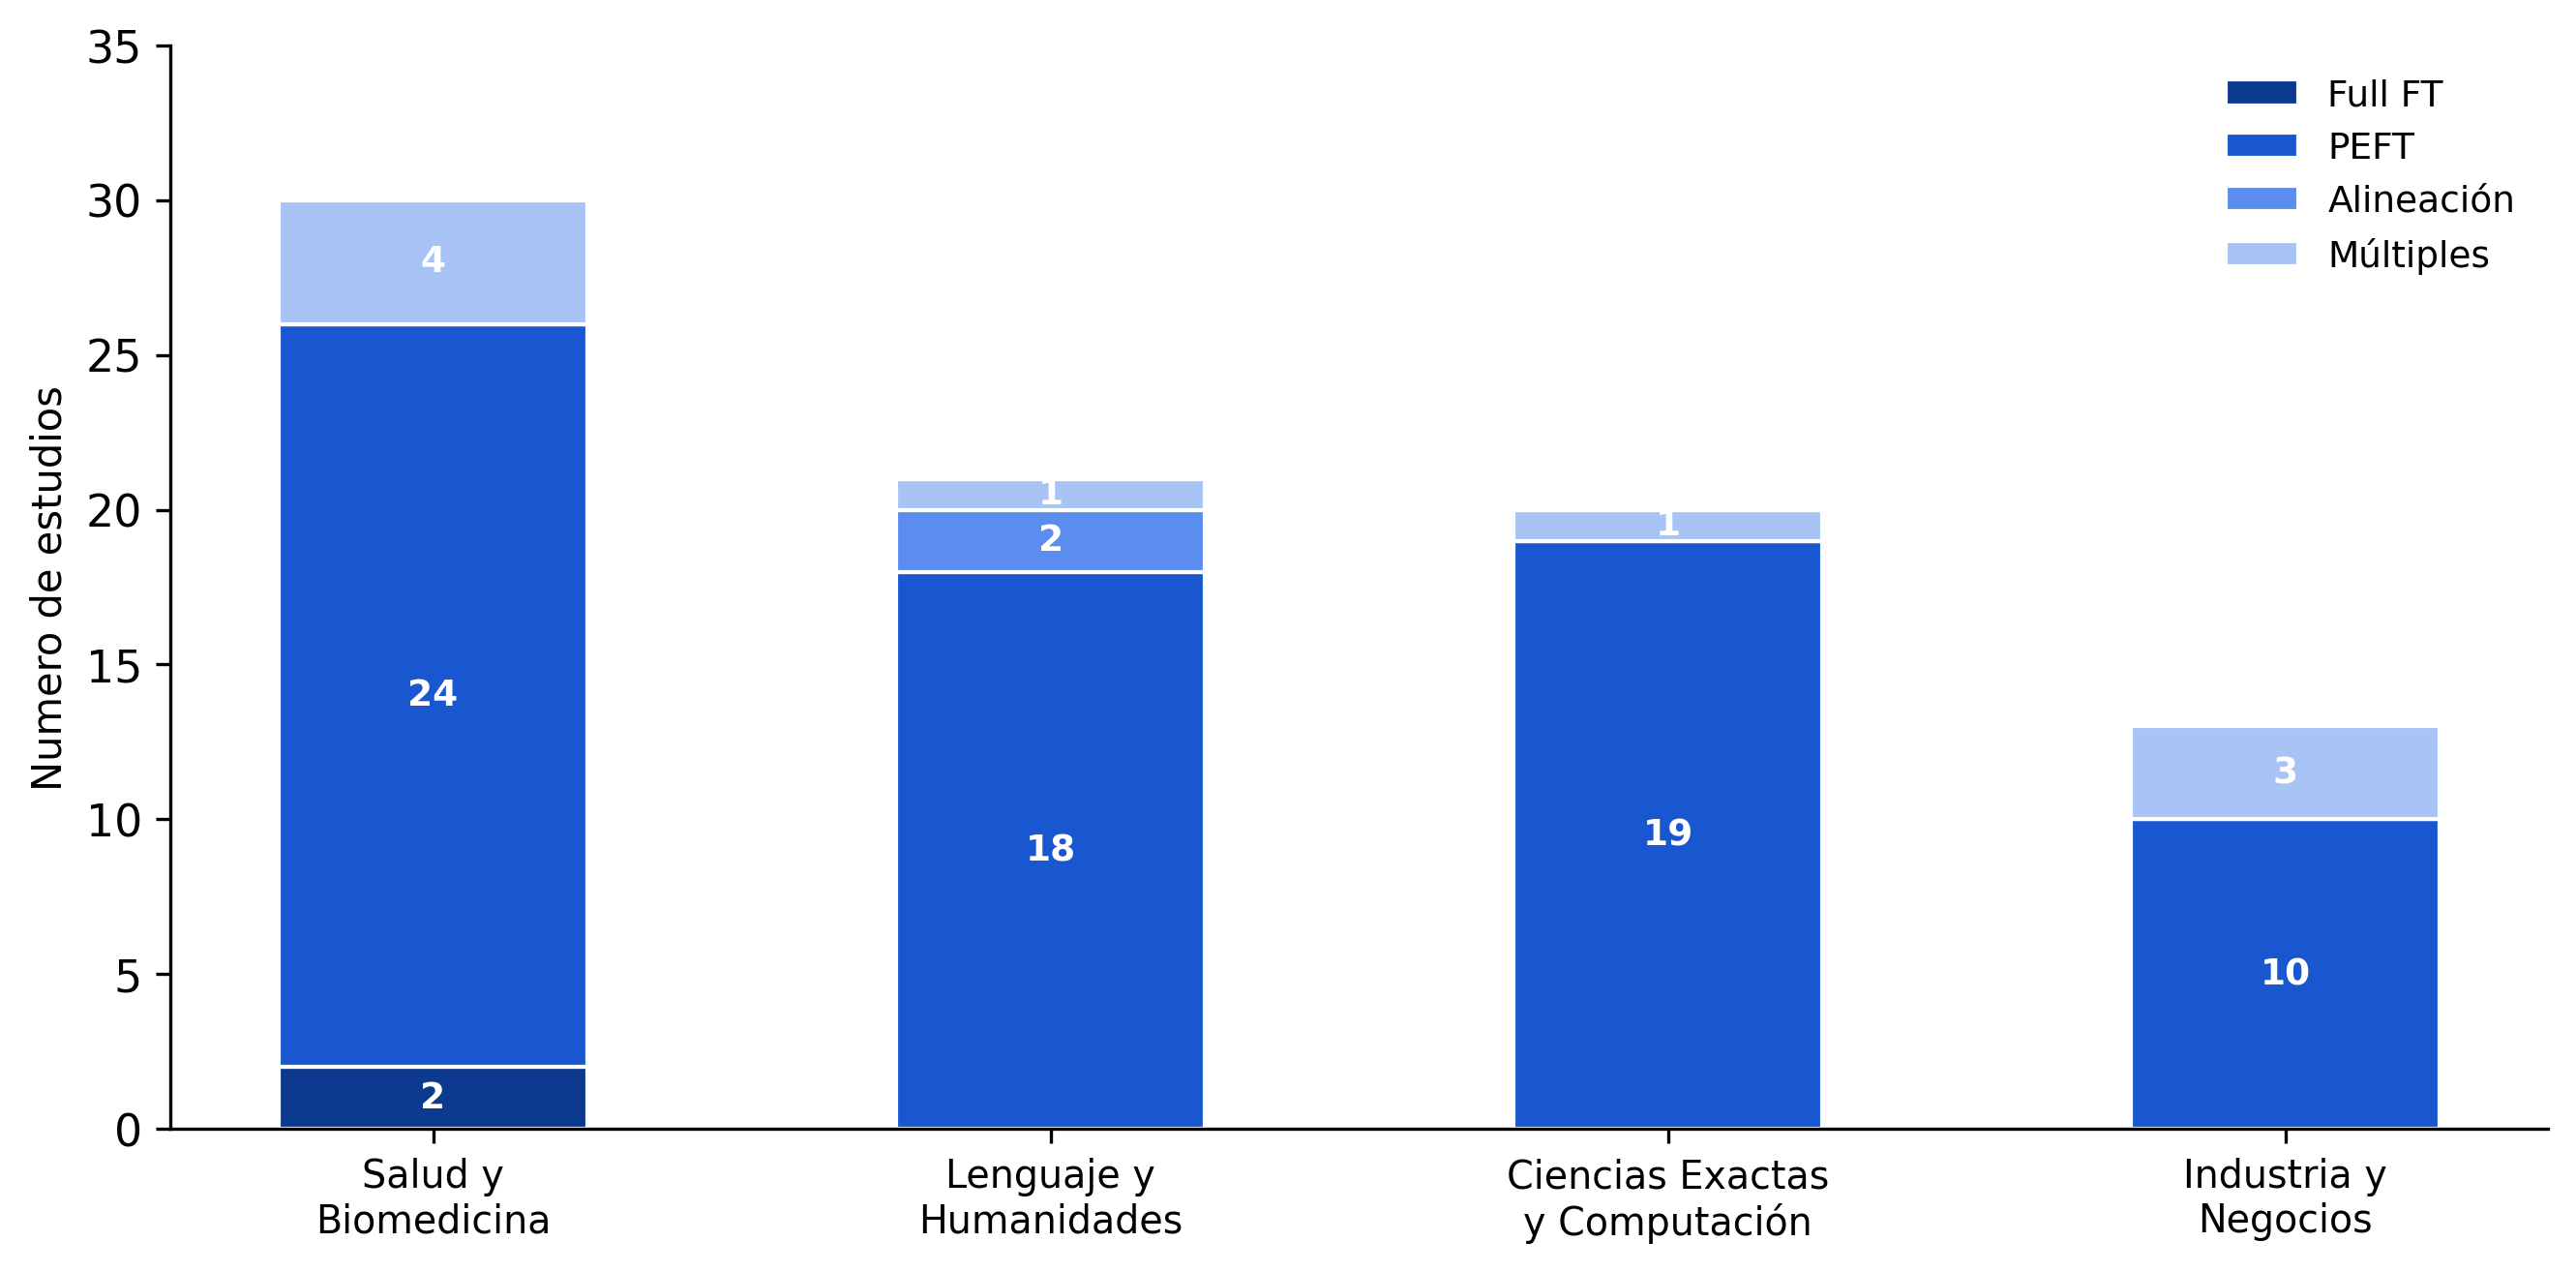
\includegraphics[width=0.9\linewidth]{Imagenes/fig4b_familias_por_dominio.png}
    \label{fig:familias}
    \begin{flushleft}
    \footnotesize
    \textit{Nota.} Las familias corresponden a las tres categorías definidas en el marco teórico: \textit{Full Fine-Tuning}, PEFT y Alineación. Un estudio puede contribuir a más de una familia si combina técnicas de distintas categorías.
    \end{flushleft}
\end{figure}

\begin{figure}[H]
    \centering
    \caption{Uso de técnicas específicas de \textit{fine-tuning} por dominio de aplicación (n = 84)}
    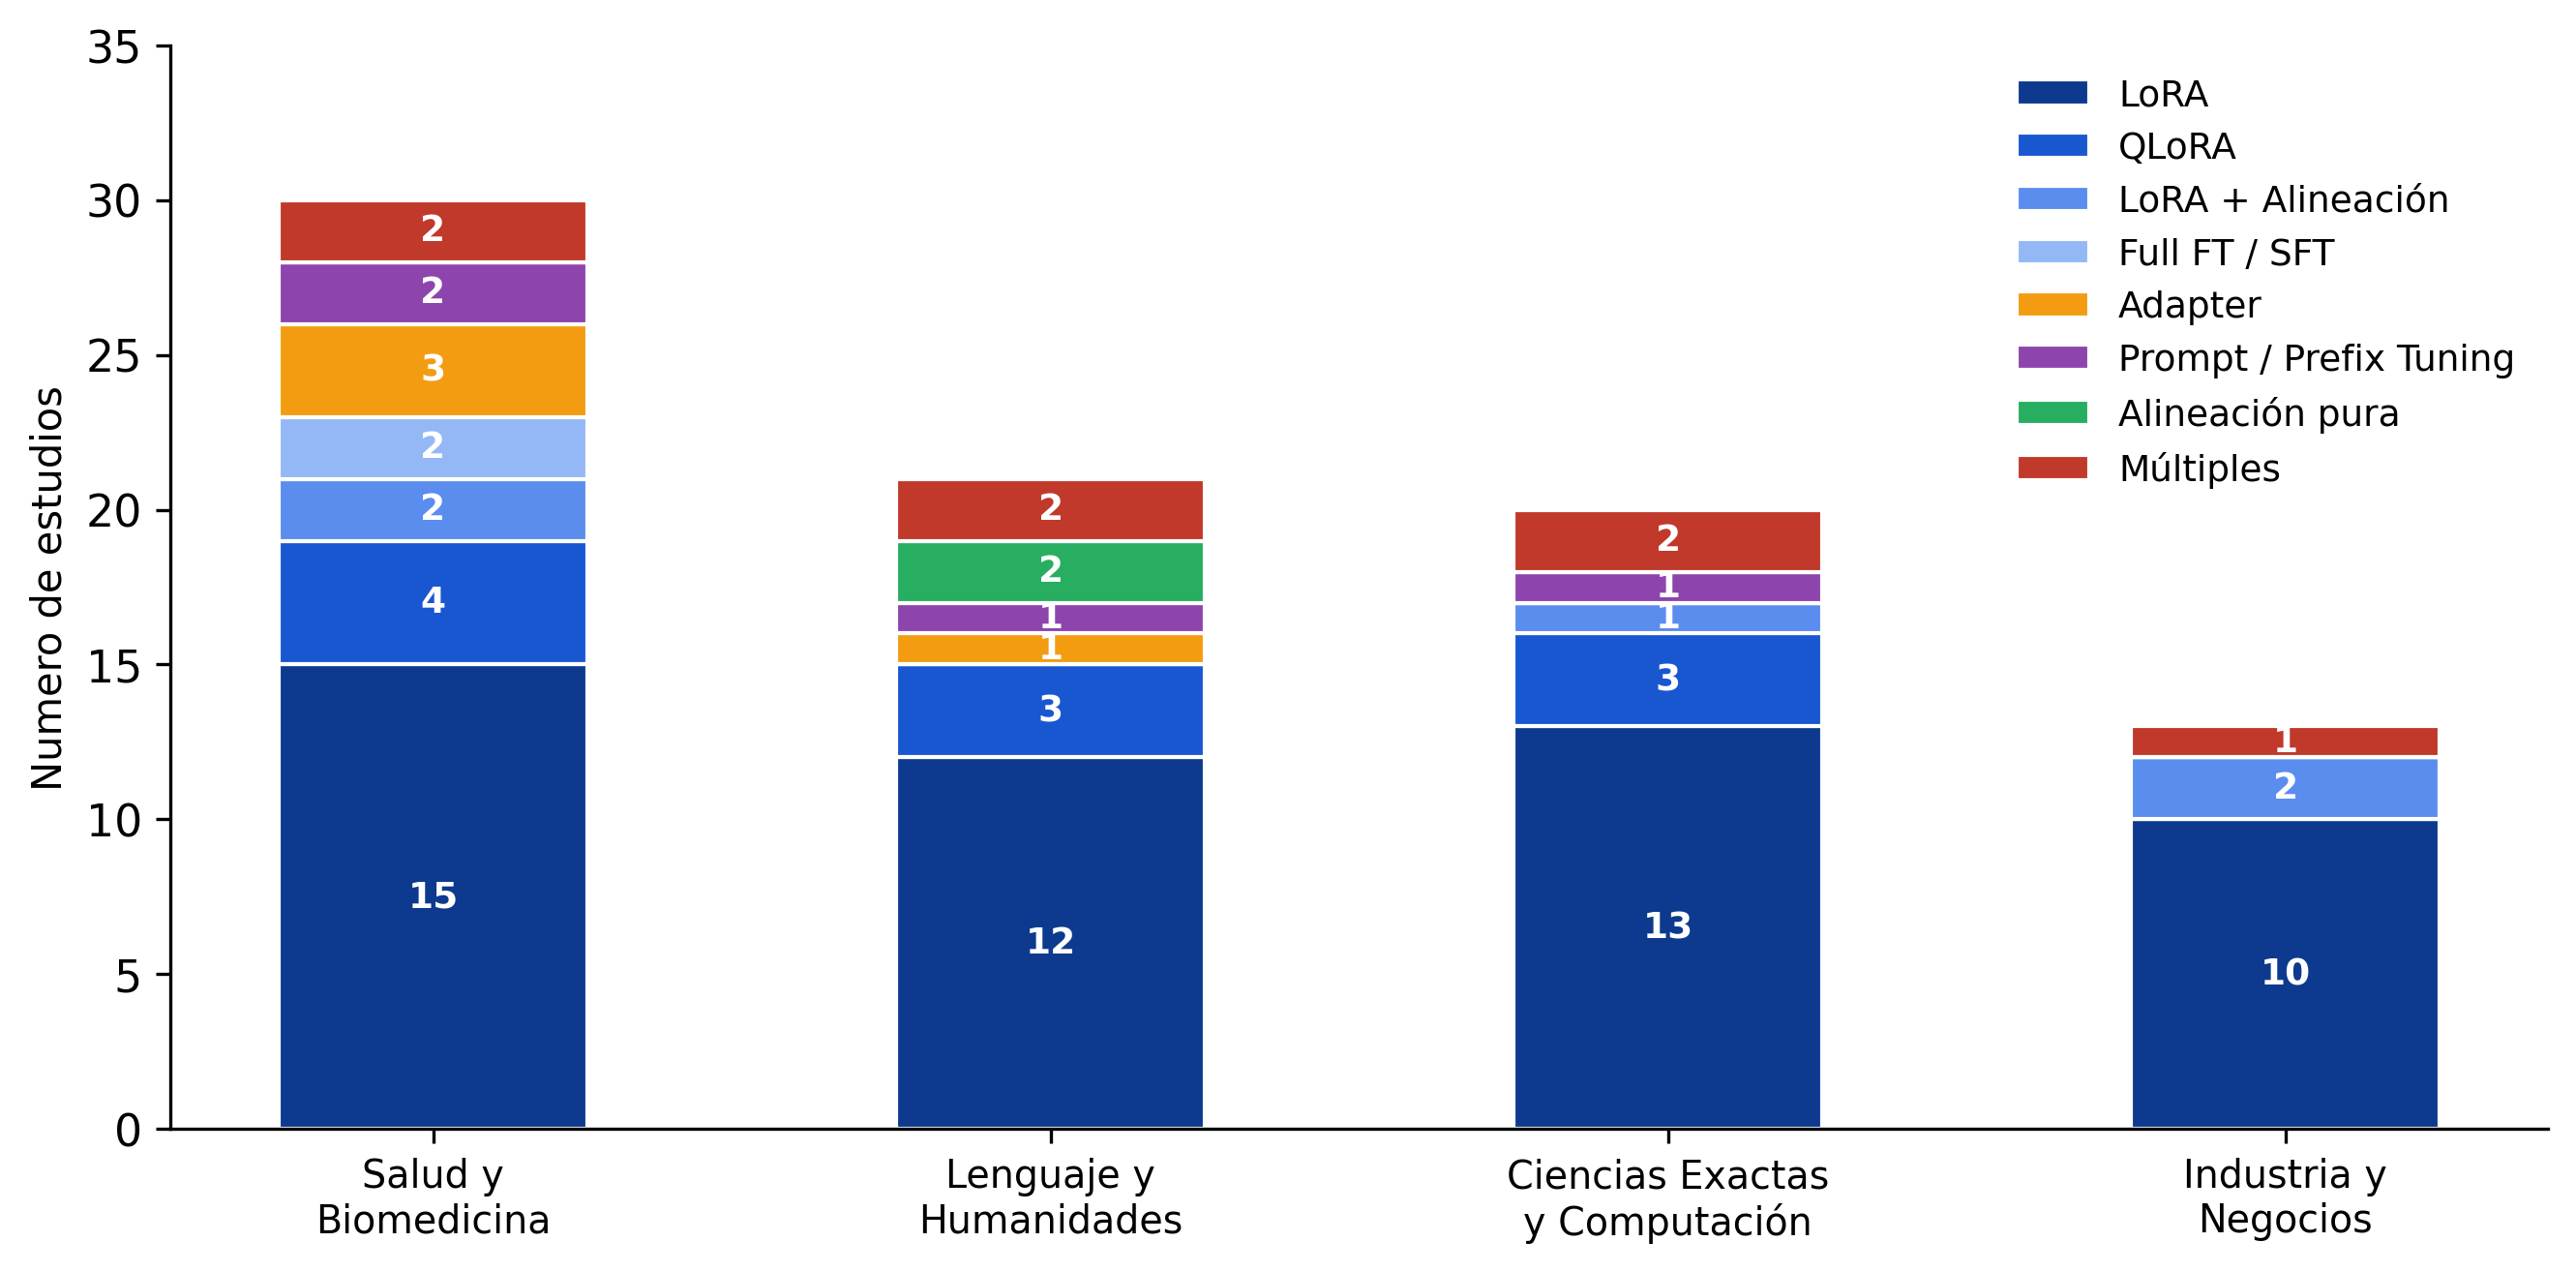
\includegraphics[width=0.9\linewidth]{Imagenes/fig4a_tecnicas_por_dominio.png}
    \label{fig:tecnicas}
    \begin{flushleft}
    \footnotesize
    \textit{Nota.} ``LoRA + Alineación'' agrupa estudios que combinan LoRA con RLHF, DPO u ORPO como mecanismo complementario. ``Alineación pura'' corresponde a estudios que aplican DPO u ORPO sin LoRA como técnica base. ``Múltiples'' agrupa estudios que combinan técnicas de distintas familias sin una técnica base dominante. Un estudio puede contabilizarse en más de una categoría si combina técnicas.
    \end{flushleft}
\end{figure}

La forma en que LoRA se combina con otras técnicas varía según el dominio. En Salud y Biomedicina aparece combinada con GRPO en reportes clínicos \parencite{kuo2025medical} y con otros mecanismos de adaptación complementaria. En Industria y Negocios predomina su combinación con RLHF para alineación \parencite{ren2025patent} y con RAG para recuperación de conocimiento especializado \parencite{xiong2025lora}. En contraste, Lenguaje y Humanidades y Ciencias Exactas y Computación presentan mayor proporción de estudios que usan LoRA de forma aislada, reflejando un carácter más experimental y comparativo \parencite{anghel2025courseeval, chen2025ft, xiang2024sumllama}.

%%%%%%%%%%%%%%%%%%%%%%%%%%%%%%%%%%%%%%%%
\subsection{Cobertura metodológica y reporte de métricas}

La proporción de estudios con pares de valores comparables (baseline y resultado explícitos) varía entre dominios. Salud y Biomedicina y Lenguaje y Humanidades presentan 9 estudios comparables cada uno (30,0\% y 42,9\% de sus respectivos dominios), Industria y Negocios 6 de 13 (46,2\%) y Ciencias Exactas y Computación 6 de 20 (30,0\%). La ausencia de valores comparables es más frecuente en dominios donde las contribuciones se centran en el diseño de sistemas o la evaluación cualitativa, como ocurre en Salud y en CyC, donde los jueces expertos o la ausencia de un único \textit{baseline} de referencia impiden el cálculo de mejora relativa.

Las métricas empleadas difieren según el dominio. F1 predomina en Salud y Biomedicina dado el énfasis en extracción de entidades y clasificación clínica \parencite{zhou2024adapter}. \textit{Accuracy} es la métrica más frecuente en Ciencias Exactas y Computación, donde los \textit{benchmarks} de razonamiento dominan \parencite{liu2025tasks}. En Lenguaje y Humanidades coexisten F1 \parencite{han2025ft}, \textit{accuracy} \parencite{kadyrbek2025dpo, shen2025ft} y métricas específicas de tarea como ROUGE-L en generación \parencite{chen2025ft}. En Industria y Negocios la heterogeneidad es máxima, con BLEU-4 \parencite{ren2025patent}, Macro-F1 \parencite{yang2025hierarchic} y ROUGE-L \parencite{song2025lora} distribuidos según la naturaleza de cada aplicación vertical.

%%%%%%%%%%%%%%%%%%%%%%%%%%%%%%%%%%%%%%%%
\subsection{Patrones transversales}

Tres patrones emergen de forma consistente a través de los cuatro dominios del corpus. La Figura~\ref{fig:mejoras} resume la dirección de los resultados reportados, mostrando que la gran mayoría de los estudios con métricas comparables reportan mejora positiva sobre sus \textit{baselines} de referencia.

\begin{figure}[H]
    \centering
    \caption{Dirección de la mejora respecto al \textit{baseline} por dominio (estudios con pares de valores comparables, n = 30)}
    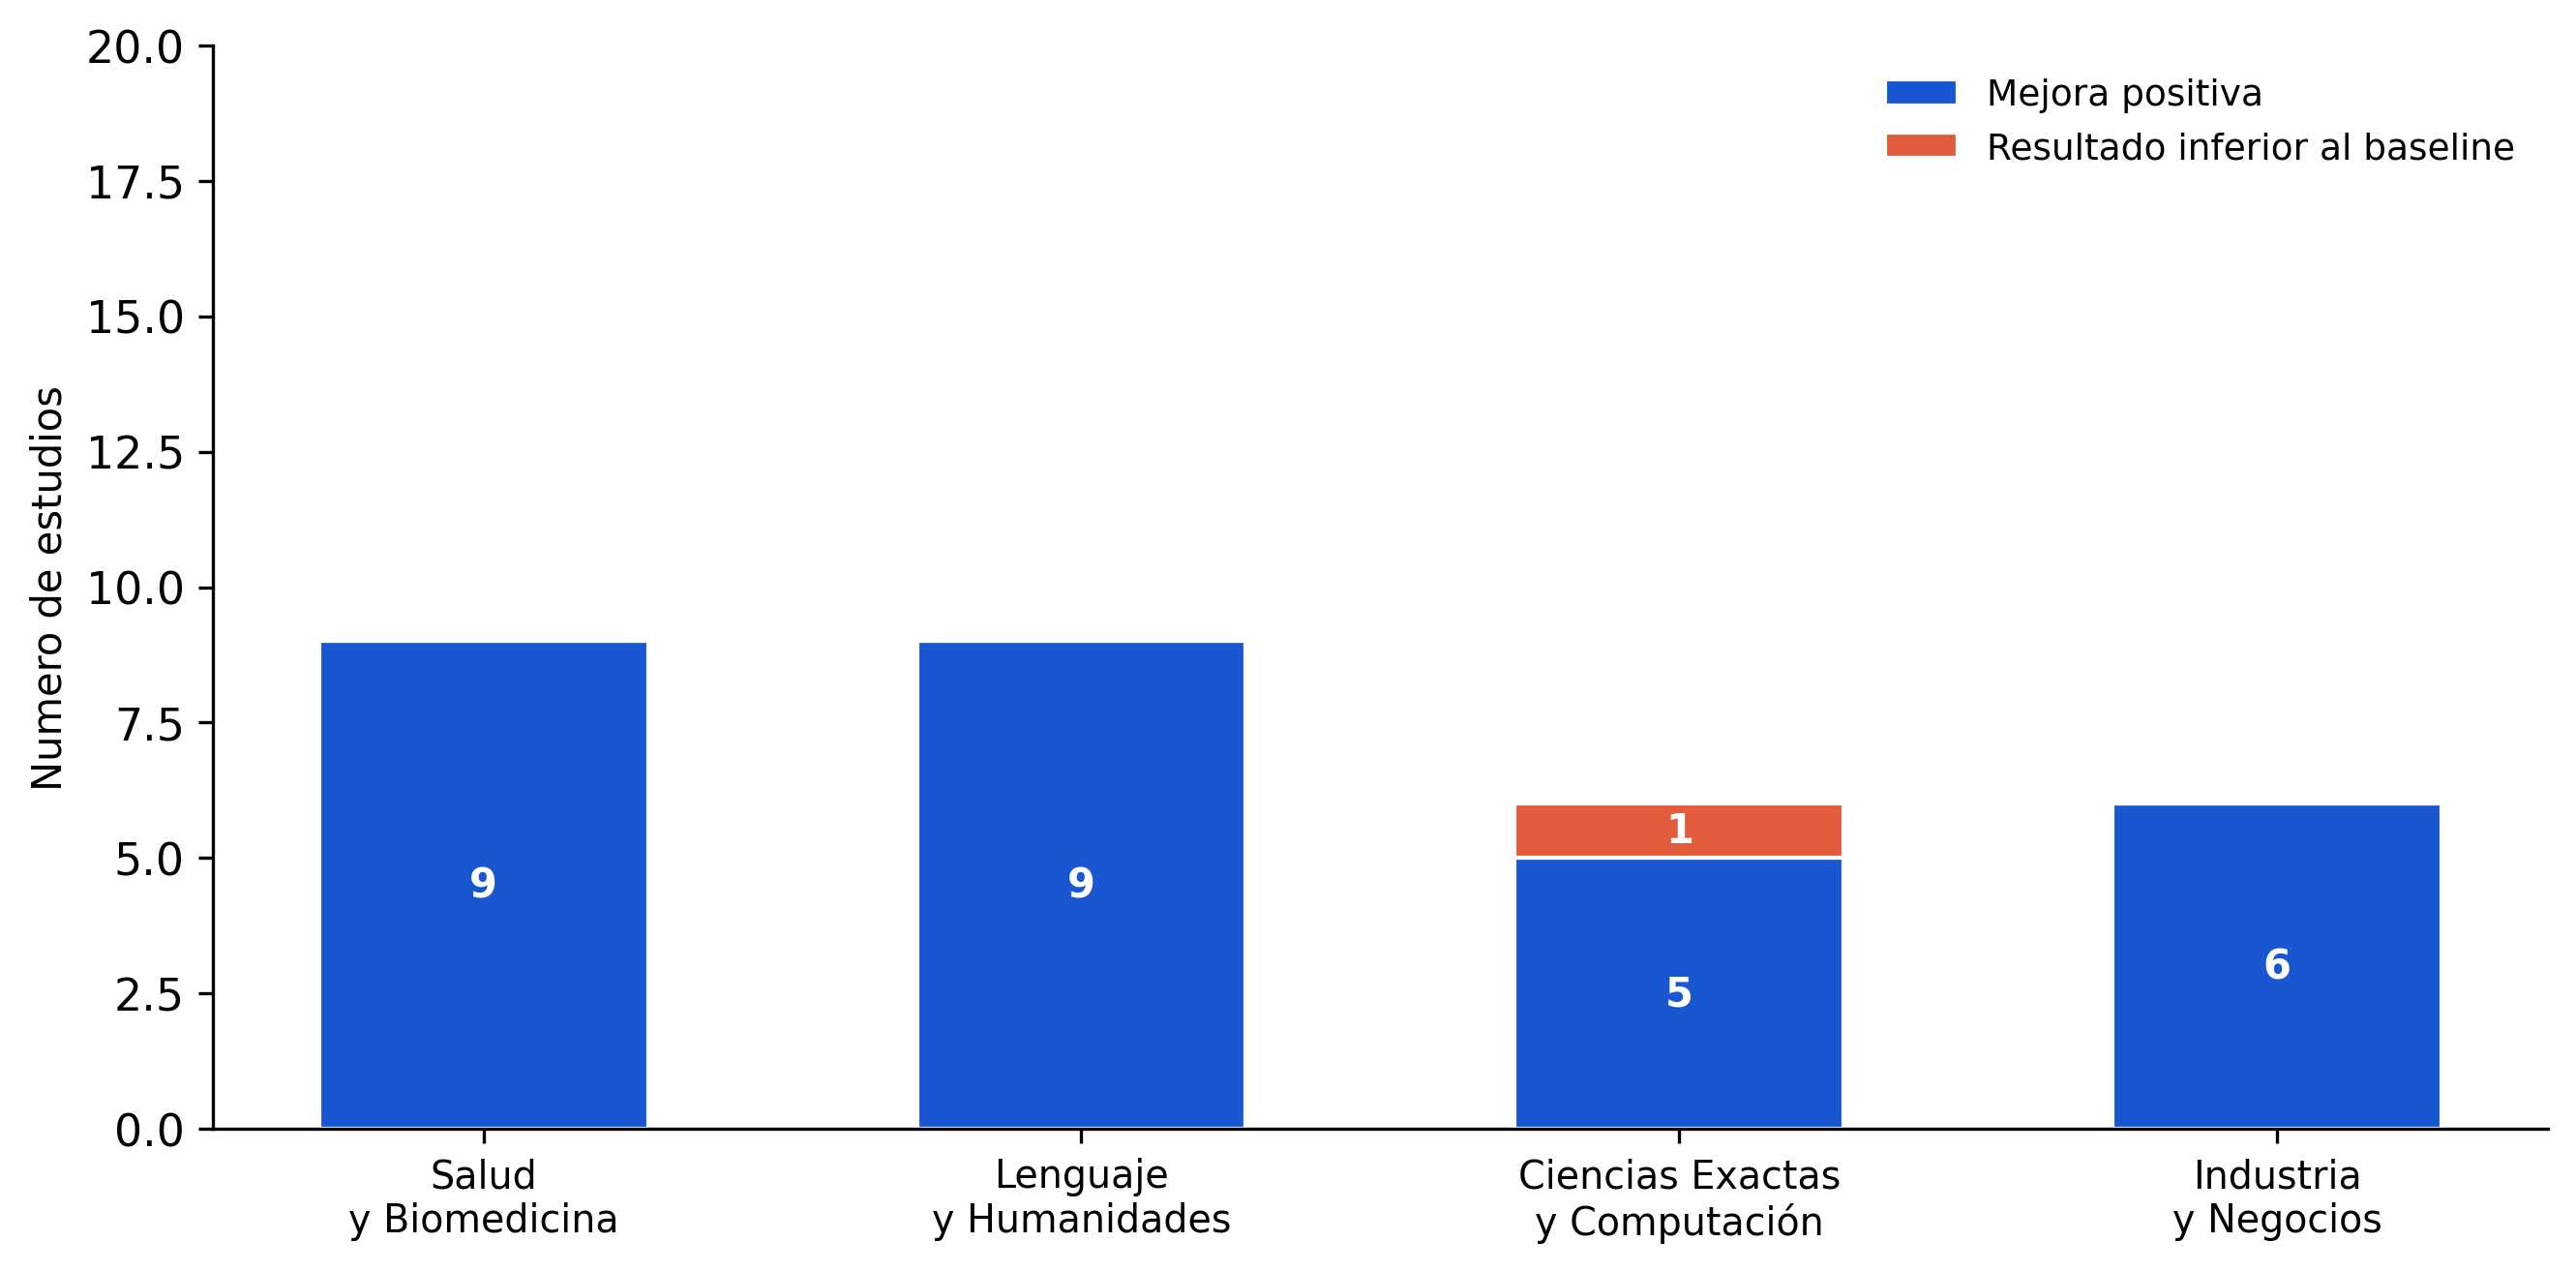
\includegraphics[width=0.9\linewidth]{Imagenes/fig5_direccion_mejoras.png}
    \label{fig:mejoras}
    \begin{flushleft}
    \footnotesize
    \textit{Nota.} Se incluyen únicamente los 30 estudios del corpus que declaran explícitamente un \textit{baseline} de referencia y reportan tanto el valor de referencia como el resultado obtenido tras el \textit{fine-tuning}, lo que permite calcular la dirección y magnitud del cambio. El único resultado negativo corresponde al dominio de Ciencias Exactas y Computación.
    \end{flushleft}
\end{figure}

El primer patrón es la dominancia transversal de LoRA como técnica de adaptación. LoRA o alguna de sus variantes está presente en 67 de los 84 estudios del corpus (79,8\%), con una frecuencia que se mantiene alta en todos los dominios sin excepción. Este patrón de adopción no depende de la tarea, el idioma ni el tamaño del modelo, lo que sugiere que LoRA ha consolidado su posición como técnica de referencia en la literatura de \textit{fine-tuning} de LLMs durante el período analizado.

El segundo patrón es la efectividad consistente del \textit{fine-tuning} sobre el modelo base sin adaptar. De los 30 estudios con pares de valores comparables, la dirección del cambio es positiva en 29 casos, con mejoras relativas que en varios estudios superan el 100\%. Este patrón se observa en dominios y tareas diversas: en diálogo geriátrico se reporta una mejora de ROUGE de 8,60\% a 34,96\% (+306,5\%) \parencite{xu2025cpel}, y en extracción de información militar una ganancia de Macro-F1 de 0,2140 a 0,7020 (+228,0\%) \parencite{yang2025hierarchic}. Es importante señalar que la heterogeneidad de métricas y \textit{datasets} entre estudios impide una agregación directa de valores absolutos; el patrón se establece a nivel de dirección de la mejora, no de magnitud promedio entre dominios.

El tercer patrón es la tendencia hacia arquitecturas compuestas en aplicaciones orientadas a producción. La familia PEFT, con LoRA como técnica predominante, no solo domina en frecuencia sino que en contextos aplicados tiende a combinarse con mecanismos complementarios: con RLHF para alineación de preferencias \parencite{ren2025patent}, con RAG para recuperación de conocimiento especializado \parencite{xiong2025lora} y con marcos de aprendizaje federado para privacidad distribuida \parencite{elbakary2025mira, liu2025federated}. Este patrón sugiere que la familia PEFT actúa como componente base sobre el que se construyen sistemas más complejos en aplicaciones de producción, especialmente en los dominios de Salud y Biomedicina e Industria y Negocios.